\documentclass[aspectratio=169]{beamer}
\mode<presentation>
%\usetheme{Warsaw}
%\usetheme{Goettingen}
\usetheme{Hannover}
%\useoutertheme{default}

%\useoutertheme{infolines}
\useoutertheme{sidebar}
\usecolortheme{dolphin}

\usepackage{amsmath}
\usepackage{amssymb}
\usepackage{enumerate}

%some bold math symbosl
\newcommand{\Cov}{\mathrm{Cov}}
\newcommand{\Cor}{\mathrm{Cor}}
\newcommand{\Var}{\mathrm{Var}}
\newcommand{\brho}{\boldsymbol{\rho}}
\newcommand{\bSigma}{\boldsymbol{\Sigma}}
\newcommand{\btheta}{\boldsymbol{\theta}}
\newcommand{\bbeta}{\boldsymbol{\beta}}
\newcommand{\bmu}{\boldsymbol{\mu}}
\newcommand{\bW}{\mathbf{W}}
\newcommand{\one}{\mathbf{1}}
\newcommand{\bH}{\mathbf{H}}
\newcommand{\by}{\mathbf{y}}
\newcommand{\bolde}{\mathbf{e}}
\newcommand{\bx}{\mathbf{x}}

\newcommand{\cpp}[1]{\texttt{#1}}

 \title{Mathematical Biostatistics Boot Camp 2: Lecture 12}
\author{Brian Caffo}
\date{\today}
\institute[Department of Biostatistics]{
  Department of Biostatistics \\
  Johns Hopkins Bloomberg School of Public Health\\
  Johns Hopkins University
}


\begin{document}
\frame{\titlepage}

%\section{Table of contents}
\frame{
  \frametitle{Table of contents}
  \tableofcontents
}

\section{Nonparametric tests}
\begin{frame}\frametitle{Nonparametric tests}
\begin{itemize}
\item ``Distribution free'' methods require fewer assumptions than
  parametric methods
\item Focus on testing rather than estimation
\item Not sensitive to outlying observations
\item Especially useful for cruder data (like ranks)
\item ``Throws away'' some of the information in the data
\item May be less powerful than parametric counterparts, when the
  parametric assumptions are true
\item For large samples, are equally efficient to parametric
  counterparts
\end{itemize}
\end{frame}

\begin{frame}
 \ttfamily \scriptsize
  \begin{tabular}{rrrrrrrrrrr}
Fish & SR  & P   & Diff & Sgn rank   & Fish & SR  & P   & Diff & Sng rank   \\ \hline
1    & .32 & .39 & .07  & +15.5  & 13   & .20 & .22 & .02  & +6.5   \\
2    & .40 & .47 & .07  & +15.5  & 14   & .31 & .30 & -.01 & -2.5   \\
3    & .11 & .11 & .00  &        & 15   & .62 & .60 & -.02 & -6.5   \\
4    & .47 & .43 & -.04 & -11.0  & 16   & .52 & .53 &  .01 & +2.5   \\
5    & .32 & .42 & .10  & +20.0  & 17   & .77 & .85 & .08  & +17.5  \\
6    & .35 & .30 & -.05 & -13.5  & 18   & .23 & .21 & -.02 & -6.5   \\
7    & .32 & .43 & .11  & +20.0  & 19   & .30 & .33 & .03  & +9.0   \\
8    & .63 & .98 & .35  & +23.0  & 20   & .70 & .57 & -.13 & -21.0  \\
9    & .50 & .86 & .36  & +24.0  & 21   & .41 & .43 &  .02 & +6.5   \\
10   & .60 & .79 & .19  & +22.0  & 22   & .53 & .49 & -.04 & -11.0  \\
11   & .38 & .33 & -.05 & -13.5  & 23   & .19 & .20 &  .01 & +2.5   \\
12   & .46 & .45 & -.01 & -2.5   & 24   & .31 & .35 & .04  & +11.0  \\
     &     &     &      &        & 25   & .48 & .40 & -.08 & -17.5  \\ \hline  
\end{tabular}\\
Measurements are mecury levels in fish (ppm)\\
Data from Rice Mathematical Statistics and Data Analysis; second edition
\normalfont \normalsize
\end{frame}

\section{Sign test}
\begin{frame}\frametitle{Alternatives to the paired t-test}
\begin{itemize}
\item Let $D_i = $ difference (\texttt{P - SR})
\item Let $\theta$ be the population median of the $D_i$
\item $H_0:\theta = 0$ versus $H_a:\theta \neq 0$ (or $>$ or $<$)
\item Notice that $\theta = 0$ iff $p = P(D > 0) = .5$ 
\item Let $X$ be the number of times $D > 0$
  \begin{itemize}
  \item $X$ is then binomial$(n,p)$
  \end{itemize}
\item The sign test tests wether $H_0:p = .5$ using $X$
\end{itemize}
\end{frame} 

\begin{frame}[fragile]\frametitle{Example}
\begin{itemize}
\item $\theta =$ median difference \texttt{p - sr}
\item $H_0:\theta = 0$ versus $H_a:\theta \neq 0$
\item Number of instances where the difference is bigger than 0 is
  15 out of 25 trials
\item \texttt{binom.test(15, 25)}
\begin{verbatim}
p-value = 0.4244
\end{verbatim}
\item Or we could have used large sample tests for a binomial
  proportion \texttt{prop.test(15, 25, p = .5)}
\begin{verbatim}
X-squared = 0.64, df = 1, p-value = 0.4237
\end{verbatim}
\end{itemize}
\end{frame}

\begin{frame}\frametitle{Discussion}
\begin{itemize}
\item Magnitude of the differences is discarded
  \begin{itemize}
  \item Perhaps too much information lost
  \end{itemize}
\item Could easily have tested $H_0:\theta = \theta_0$ by calculating the number
  of times $D > \theta_0$ and performing a binomial test
  \begin{itemize}
  \item We can invert these tests to get a distribution free confidence interval
    for the median
  \end{itemize}
\end{itemize}
\end{frame}

\section{Signed rank test}
\begin{frame}\frametitle{Signed rank test}
\begin{itemize}
\item Wilcoxon's statistic uses the information in the {\bf signed ranks}
  of the differences
\item Saves some of the information regarding the magnitude of the differences
\item Still tests $H_0:\theta = 0$ versus the three alternatives
\item Appropriately normalized, the test statistic follows a normal distribution
\item Also the exact small sample distribution of the signed rank statistic is known
  (if there are no ties)
\end{itemize}
\end{frame}

\begin{frame}\frametitle{Signed rank procedure}
\begin{enumerate}
\item Take the paired differences
\item Take the absolute values of the differences
\item Rank these absolute values, throwing out the 0s
\item Multiply the ranks by the sign of the difference (+1 for a positive difference and -1 for
  a negative difference)
\item Cacluate the rank sum $W_+$ of the positive ranks
\end{enumerate}
\end{frame}

\begin{frame}\frametitle{Signed rank procedure}
\begin{itemize}
\item If $\theta > 0$ then $W_+$ should be large 
\item If $\theta < 0$ then $W_+$ should be small 
\item Properly normalized, $W_+$ follows a large sample normal distribution
\item For small sample sizes, $W_+$ has an exact distribution under the null hypothesis
\item Can get critical values from tables in the textbook
\end{itemize}
\end{frame}

\section{Monte Carlo}
\begin{frame}\frametitle{Monte Carlo}
\begin{itemize}
\item Assume no ties
\item Simulate $n$ observations from any distribution that has $\theta = 0$ as
  its median
\item Rank the absolute value of the data, retain the signs, calculate
  the signed rank statistic
\item Apply this procedure over and over, the proportion of time that
  the observed test statistic is larger or smaller (depending on the hypothesis)
  is a Monte Carlo approximation to the P-value
\end{itemize}
\end{frame}

\begin{frame}\frametitle{Monte Carlo}
\begin{itemize}
\item Here's a slightly more elegant way to simulate from the null distribution
\item Consider the ranks $1,\ldots,n$
\item Randomly assign the signs as binary with probability $.5$ of
  being positive and $.5$ of being negative
\item Calculate the signed rank statistic
\item Apply this procedure over and over, the proportion of time that
  the observed test statistic is larger or smaller (depending on the hypothesis)
  is a Monte Carlo approximation to the P-value
\end{itemize}
\end{frame}


\begin{frame}\frametitle{Large sample distribution of $W_+$}
\begin{itemize}
\item Under $H_0$ and if there are no ties 
  \begin{itemize}
  \item $E(W_+) = n(n+1)/4$
  \item $Var(W_+) = n(n+1)(2n+1)/24$
  \item $TS = \{W_+ - E(W_+)\}/Sd(W_+) \rightarrow \mathrm{Normal}(0, 1)$
  \end{itemize}
\item There is a correction term necessary for ties
\item Without ties, it's possible to do an exact (small sample) test
\end{itemize}
\end{frame}

\begin{frame}[fragile]\frametitle{Example}
\begin{verbatim}
diff <- c(.07, .07, .00, -.04,  ...)
wilcox.test(diff, exact = FALSE)
\end{verbatim}
\begin{itemize}
\item $H_0:\mbox{Med diff} = 0$ vesus $H_a:\mbox{Med diff} \neq 0$
\item $W_+ = 194.5$
\item $E(W_+) = 24 \times 25 / 4 = 150$
\item $\Var(W_+) = 24 \times 25 \times 49 / 24 = 1,225$
\item $TS = (194.5 - 150) / \sqrt{1,224} = 1.27$
\item P-value $=.20$
\item R's P-value (uses correction for ties) $= 0.21$
\end{itemize}
\end{frame}

\section{Independent groups}
\begin{frame}\frametitle{Methods for unpaired samples} 
Comparing two measuring techniques A and B\\
Units are in deg C per gram
\begin{center}
\ttfamily
  \begin{tabular}{|cc|c|} \hline
\multicolumn{2}{|c|}{Method A} & Method B \\ \hline
79.98 & 80.05 & 80.02 \\
80.04 & 80.03 & 79.94 \\
80.02 & 80.02 & 79.98 \\
80.04 & 80.00 & 79.97 \\
80.03 & 80.02 & 79.97 \\
80.03 &       & 80.03 \\
80.04 &       & 79.95 \\
79.97 &       & 79.97 \\ \hline
  \end{tabular}
\end{center}
Data from Rice Mathematical Statistics and Data Analysis; second edition \normalsize \normalfont
\end{frame}

\section{Mann/Whitney test}
\begin{frame}\frametitle{The Mann/Whitney test}
\begin{itemize}
\item Tests whether or not the two treatments have the same location
\item Assumes independent identically distributed errors, not necessarily normal
\item Null hypothesis can also be written more generally as a stochastic shift for
  two arbitrary distributions
\item Test uses the sum of the ranks obtained by discarding the
  treatment labels
\item Also called the Wilcoxon rank sum test
\end{itemize}
\end{frame}


\begin{frame}\frametitle{The Mann-Whitney test}
\begin{itemize}
\item Procedure
  \begin{enumerate}
  \item Discard the treatment labels
  \item Rank the observations 
  \item Calculate the sum of the ranks in the first treatment
  \item Either 
    \begin{itemize}
    \item calculate the asymptotic normal distrubtion of 
      this statistic
    \item compare with the exact distribution under the null hypothesis
    \end{itemize}
\end{enumerate}
\end{itemize}
\end{frame}

\begin{frame}
\begin{center}
\ttfamily
  \begin{tabular}{|cc|c|} \hline
\multicolumn{2}{|c|}{Method A} & Method B \\ \hline
 7.5  & 21.0  & 11.5  \\
19.0  & 15.5  &  1.0  \\
11.5  & 11.5  &  7.5  \\
19.0  &  9.0  &  4.5  \\
15.5  & 11.5  &  4.5  \\
15.5  &       & 15.5  \\
19.0  &       &  2.0  \\
 4.5  &       &  4.5  \\ \hline
\multicolumn{2}{|c|}{180} & 51 \\ \hline
  \end{tabular}
\end{center}
Sum has to add up to $21 \times 22 / 2 = 231$ \normalsize \normalfont
\end{frame}

\begin{frame}[fragile]\frametitle{Aside}
Gauss supposedly came up with this in grade school
\begin{verbatim}
  x =   1  +    2  +    3  +    4  +  ...  +    n
  x =   n  +  n-1  +  n-2  +  n-3  +  ...  +    1

Therefore
  2x = n+1  +  n+1  +  n+1  +  n+1  +  ...  +  n+1

So 2x = n (n + 1) / 2

So x = n (n + 1) / 2
\end{verbatim}
\end{frame}

\begin{frame}\frametitle{Results} 
\begin{itemize}
\item  Let $W$ be the sum of the ranks for the first treatment ($A$)
\item Let $n_A$ and $n_B$ be the sample sizes 
\item Then
\begin{itemize}
\item $E(W) = n_A ( n_A + n_B + 1)/ 2$
\item $\Var(W) = n_A n_B (n_A + n_B + 1) / 12$
\item $TS = \{W - E(W)\}/Sd(W) \rightarrow N(0,1)$
\end{itemize}
\item Also the exact distribution of $W$ can be calculated
\end{itemize}
\end{frame}

\begin{frame}\frametitle{Example}
\begin{itemize}
\item $W = 51$
\item $E(W) = 8 (8 + 13 + 1) / 2 = 88$
\item $Sd(W) = \sqrt{8 \times 13 (8 + 13 + 1) / 12} = 13.8$
\item $TS = (51 - 88) / 13.8 = -2.68$
\item Two-sided P-value$ = .007$
\item R function \texttt{wilcox.test} will perform the test
\end{itemize}
\end{frame}

\section{Monte Carlo}
\begin{frame}\frametitle{Monte Carlo}
\begin{itemize}
\item Note that under $H_0$, the two groups are {\bf exchangeable}
\item Therefore, any allocation of the ranks between the two groups is
  equally likely
\item Procedure: Take the ranks $1,\ldots,N_A+N_B$ and permute them
\item Take the first $N_A$ ranks and allocate them to Group $A$;
  allocate the remainder to Group $B$
\item Calculate the test statistic
\item Repeat this process over and over; the proportion of times the
  test statistic is larger or smaller (depending on the alternative) than
  the observed value is an exact P-value
\end{itemize}
\end{frame}

\begin{frame}\frametitle{Notes about nonpar tests}
\begin{itemize}
\item Tend to be more robust to outliers than parametric counterparts
\item Do not require normality assumptions
\item Usually have exact small-sample versions
\item Are often based on ranks rather than the raw data
\item Loss in power over parametric counterparts is often not bad
\item Nonpar tests are not assumption free
\end{itemize}
\end{frame}

\section{Permutation tests}
\begin{frame}\frametitle{Permutation tests}
  \begin{itemize}
  \item Permutation tests are similar to the rank-sum tests, though they use the
    actual data rather than the ranks
  \item That is, consider the null hypothesis that the distribution of the
    observations from each group is the same
  \item Then, the group labels are irrelevant
  \item We then discard the group levels and permute the combined data
  \item Split the permuted data into two groups with $n_A$ and $n_B$
    observations (say by always treating the first $n_A$ observations as
    the first group)
  \item Evaluate the probability of getting a statistic as large or
    large than the one observed
  \item An example statistic would be the difference in the averages between the two groups;
    one could also use a t-statistic 
  \end{itemize}
\end{frame}

\begin{frame}
  \begin{itemize}
  \item This is an easy way to produce a null distribution for a test of equal distributions
  \item Similar in flavor to the bootstrap
  \item This procedure produces an exact test
  \item Less robust, but more powerful than the rank sum tests
  \item Very popular in genomic applications
  \end{itemize}
\end{frame}

\begin{frame}
  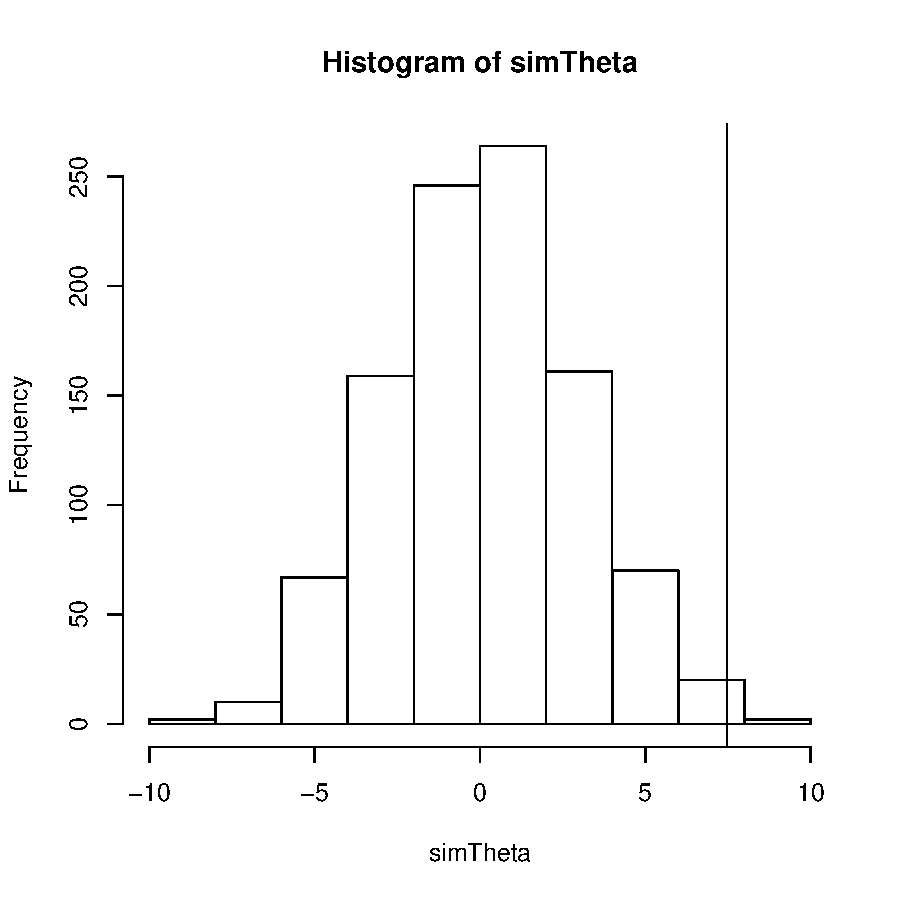
\includegraphics[width=3in]{permute.pdf}
\end{frame}



\end{document}
